% Gabarit pandoc des corrigés publiés (brut et guidé). Contenu sans marque ni nom de site.
% Compilation : lualatex (latexmk -lualatex).
% Le Markdown reste la source unique : ne pas éditer ce fichier .tex à la main.
\documentclass[11pt,a4paper]{article}

% --- Moteur, polices (Latin Modern) et langue ---------------------------------
\usepackage{iftex}
\ifLuaTeX\else\errmessage{Ce document se compile avec lualatex}\fi
\usepackage{amsmath,amssymb,mathtools}
\usepackage{fontspec}
% mathrm=sym : \mathrm prend ses glyphes dans la police mathématique (ℓ, μ, Ω), comme KaTeX.
\usepackage[math-style=TeX,bold-style=TeX,mathrm=sym]{unicode-math}
% Repli pour les glyphes absents de Latin Modern (indices et exposants Unicode,
% flèches, filets des schémas en texte, symboles) : DejaVu, puis Latin Modern Math
% (ℓ, lettres mathématiques Unicode des légendes).
\directlua{
  luaotfload.add_fallback("repliTexte", {"DejaVuSerif:mode=harf;", "DejaVuSans:mode=harf;", "file:latinmodern-math.otf:mode=harf;"})
  luaotfload.add_fallback("repliMono", {"DejaVuSansMono:mode=harf;", "DejaVuSans:mode=harf;", "file:latinmodern-math.otf:mode=harf;"})
}
\setmainfont{Latin Modern Roman}[RawFeature={fallback=repliTexte}]
\setsansfont{Latin Modern Sans}[RawFeature={fallback=repliTexte}]
\setmonofont{Latin Modern Mono}[RawFeature={fallback=repliMono}]
\setmathfont{Latin Modern Math}
\usepackage[french]{babel}
\frenchsetup{SmallCapsFigTabCaptions=false}

% --- Mise en page --------------------------------------------------------------
\usepackage[a4paper,margin=2.2cm,headheight=14pt,footskip=1.2cm]{geometry}
\usepackage{microtype}
\setlength{\emergencystretch}{4em}
\tolerance=1500
\setlength{\parindent}{0pt}
\setlength{\parskip}{0.55\baselineskip plus 2pt minus 1pt}
\usepackage{xcolor}
% Gris nommés : babel-french rend « ! » actif dans le document.
\definecolor{gris2}{gray}{0.98}
\definecolor{gris3}{gray}{0.97}
\definecolor{gris5}{gray}{0.95}
\definecolor{gris35}{gray}{0.65}
\definecolor{gris40}{gray}{0.60}
\definecolor{gris45}{gray}{0.55}
\definecolor{gris50}{gray}{0.50}
\definecolor{gris55}{gray}{0.45}
\definecolor{gris60}{gray}{0.40}
\definecolor{gris65}{gray}{0.35}
\definecolor{gris70}{gray}{0.30}
\definecolor{gris80}{gray}{0.20}
\definecolor{gris85}{gray}{0.15}
\usepackage{graphicx}
\usepackage{float}
\usepackage{caption}
\captionsetup{font=small,labelformat=empty,justification=centering}
\usepackage{booktabs,longtable,array,multirow,calc}
\usepackage{siunitx}
\sisetup{locale=FR}
\usepackage[version=4]{mhchem}
\usepackage{listings}
\usepackage{fancyhdr}
\usepackage{lastpage}
\usepackage[most]{tcolorbox}
\usepackage{enumitem}
\setlist{nosep,leftmargin=*,topsep=2pt}
\usepackage[hidelinks,unicode]{hyperref}
\usepackage{bookmark}
\hypersetup{pdftitle={Centrale-Supélec MP-MPI — Mathématiques 1 2026},pdfauthor={Rédigé par IA},pdfcreator={LaTeX},pdfsubject={Corrigé brut}}
\usepackage{xurl}

% --- Pandoc : listes, tableaux, figures ----------------------------------------
\providecommand{\passthrough}[1]{#1}
\providecommand{\tightlist}{\setlength{\itemsep}{0pt}\setlength{\parskip}{0pt}}

\makeatletter
\def\maxwidth{\ifdim\Gin@nat@width>\linewidth\linewidth\else\Gin@nat@width\fi}
\def\maxheight{\ifdim\Gin@nat@height>0.55\textheight 0.55\textheight\else\Gin@nat@height\fi}
\makeatother
\setkeys{Gin}{width=\maxwidth,height=\maxheight,keepaspectratio}
\setcounter{secnumdepth}{-\maxdimen}
\providecommand{\pandocbounded}[1]{#1}

% --- Code (listings) -----------------------------------------------------------
\lstset{
  basicstyle=\ttfamily\small,
  columns=fullflexible,
  keepspaces=true,
  breaklines=true,
  breakatwhitespace=false,
  postbreak=\mbox{\textcolor{gris50}{$\hookrightarrow$}\space},
  frame=single,
  rulecolor=\color{gris35},
  framesep=4pt,
  xleftmargin=5pt,xrightmargin=5pt,
  backgroundcolor=\color{gris3},
  keywordstyle=\bfseries,
  commentstyle=\color{gris65},
  stringstyle=\color{gris80},
  showstringspaces=false,
  tabsize=4,
  extendedchars=true,
  aboveskip=6pt,belowskip=6pt,
}

% --- Macros des corrigés (KaTeX ↔ LaTeX) ---------------------------------------
% Les corrigés sont écrits pour KaTeX : on définit ici ce que KaTeX connaît et
% que LaTeX n'a pas, sans jamais retoucher le Markdown.
\providecommand{\R}{\mathbb{R}}
\providecommand{\N}{\mathbb{N}}
\providecommand{\Z}{\mathbb{Z}}
\providecommand{\Q}{\mathbb{Q}}
\providecommand{\C}{\mathbb{C}}
\providecommand{\dd}{\mathrm{d}}
\providecommand{\llbracket}{\lBrack}
\providecommand{\rrbracket}{\rBrack}
\providecommand{\lBrace}{\lbrace}
\providecommand{\rBrace}{\rbrace}
\providecommand{\Box}{\square}
\providecommand{\Diamond}{\lozenge}
\providecommand{\varnothing}{\emptyset}
\providecommand{\argmax}{\operatorname*{arg\,max}}
\providecommand{\argmin}{\operatorname*{arg\,min}}
\renewcommand{\leq}{\leqslant}
\renewcommand{\geq}{\geqslant}

% Équation hors texte : réduite à la largeur de la ligne si elle déborde.
\newsavebox{\boiteequation}
\newcommand{\equationajustee}[1]{%
  \sbox{\boiteequation}{$\displaystyle #1$}%
  \ifdim\wd\boiteequation>\linewidth
    \[\resizebox{\linewidth}{!}{\usebox{\boiteequation}}\]%
  \else
    \[#1\]%
  \fi}

% --- Encadrés pédagogiques (sobres, lisibles en noir et blanc) -----------------
\tcbset{
  encadre/.style={
    enhanced,breakable,sharp corners,
    colback=white,colframe=gris55,
    boxrule=0.4pt,leftrule=2.2pt,
    left=6pt,right=6pt,top=3pt,bottom=3pt,
    before skip=6pt,after skip=6pt,
    fonttitle=\bfseries\small,coltitle=black,
    attach title to upper,after title={\quad},
    parbox=false,
  }
}
\newtcolorbox{indication}[1]{encadre,colframe=gris45,colback=gris2,title={Indication~#1}}
\newtcolorbox{methode}{encadre,colframe=gris70,title={Méthode}}
\newtcolorbox{piege}{encadre,colframe=gris85,boxrule=0.8pt,leftrule=2.2pt,title={Piège}}
\newtcolorbox{jury}{encadre,colframe=gris60,colback=gris5,title={Jury}}
\newtcolorbox{encadrenote}{encadre,colframe=gris40}

% --- Titres de section ---------------------------------------------------------
\usepackage{titlesec}
\titleformat{\section}{\Large\bfseries}{}{0pt}{}
\titleformat{\subsection}{\large\bfseries}{}{0pt}{}
\titleformat{\subsubsection}{\normalsize\bfseries}{}{0pt}{}
\titlespacing*{\section}{0pt}{14pt plus 4pt minus 2pt}{6pt}
\titlespacing*{\subsection}{0pt}{10pt plus 3pt minus 2pt}{4pt}
\titlespacing*{\subsubsection}{0pt}{8pt plus 2pt minus 2pt}{2pt}

% --- En-tête et pied de page ---------------------------------------------------
\pagestyle{fancy}
\fancyhf{}
\fancyhead[L]{\small\textsc{Corrigé brut} · Centrale-Supélec MP-MPI}
\fancyhead[R]{\small Maths 1 2026}
\fancyfoot[L]{\footnotesize Corrigé rédigé par IA, non officiel}
\fancyfoot[R]{\footnotesize \thepage\,/\,\pageref*{LastPage}}
\renewcommand{\headrulewidth}{0.4pt}
\renewcommand{\footrulewidth}{0pt}
\fancypagestyle{plain}{\fancyhf{}\fancyfoot[R]{\footnotesize \thepage\,/\,\pageref*{LastPage}}\fancyfoot[L]{\footnotesize Corrigé rédigé par IA, non officiel}\renewcommand{\headrulewidth}{0pt}}

\begin{document}
\thispagestyle{plain}
\begin{center}
  {\small\scshape Corrigé brut}\par\smallskip
  {\LARGE\bfseries Centrale-Supélec MP-MPI — Mathématiques 1 2026\par}\medskip
  {\large Centrale-Supélec · MP-MPI · Maths 1 · 2026\par}
\end{center}
\vspace{2pt}\hrule\vspace{8pt}

\emph{Corrigé rédigé par IA, non officiel. Signalez toute erreur.}

\textbf{Sur quelques sous-groupes de \({\mathrm{GL}}_n(\mathbb{R})\).} Épreuve de 4 heures, calculatrice autorisée. Trois parties indépendantes. Notations : \(E_{k\ell}\) désigne la base canonique de \({\mathcal{M}}_n(\mathbb{R})\) et \(\|M\|=\sqrt{\operatorname{tr}(M^\top M)}\) la norme euclidienne canonique de \({\mathcal{M}}_n(\mathbb{R})\) (toutes les normes y sont équivalentes).

Trois énoncés ne sont pas exacts tels quels : \textbf{Q6.a} (il manque l'hypothèse \(2\pi\in\theta\mathbb{Z}+\theta'\mathbb{Z}\)), \textbf{Q38} (la majoration \(|z|\leqslant|ij|\) est fausse en général) et \textbf{Q39} (il faut que \(k\) soit du signe de \(ij\)). Chaque fois, un contre-exemple est donné et la conclusion utile pour la suite est démontrée.

\begin{center}\rule{0.5\linewidth}{0.5pt}\end{center}

\hypertarget{partie-a-sous-groupes-finis-de-mathrmo_nmathbbr}{%
\section{\texorpdfstring{Partie A --- Sous-groupes finis de \({\mathrm{O}}_n(\mathbb{R})\)}{Partie A --- Sous-groupes finis de \{\textbackslash mathrm\{O\}\}\_n(\textbackslash mathbb\{R\})}}\label{partie-a-sous-groupes-finis-de-mathrmo_nmathbbr}}

\hypertarget{i-guxe9nuxe9ralituxe9s}{%
\subsection{I --- Généralités}\label{i-guxe9nuxe9ralituxe9s}}

\hypertarget{q1}{%
\subsubsection{Q1}\label{q1}}

Supposons \(G\) fini, de cardinal \(N\geqslant 1\).

\emph{Trace.} \(\operatorname{tr}G\) est l'image de l'ensemble fini \(G\) par l'application \(\operatorname{tr}\), donc \(|\operatorname{tr}G|\leqslant N\) : \textbf{\(\operatorname{tr}G\) est fini.}

\emph{Exposant.} Soit \(x\in G\). Le sous-groupe \(\langle x\rangle\subset G\) est fini, donc \(x\) est d'ordre fini \(d_x=|\langle x\rangle|\).

L'ordre d'un élément d'un groupe fini divise le cardinal du groupe : \(d_x\mid N\). En écrivant \(N=d_xq\), on obtient

\equationajustee{x^N=(x^{d_x})^q=I_n.}

Avec \(m=N\in{\mathbb{N}}^*\), indépendant de \(x\), on a \(x^m=I_n\) pour tout \(x\in G\) : \textbf{\(G\) est d'exposant fini.}

(Sans ce théorème, \(m=\operatorname{ppcm}(d_x)_{x\in G}\), ou \(m=N!\), convient aussi, puisque chaque \(d_x\leqslant N\).)

\hypertarget{q2}{%
\subsubsection{Q2}\label{q2}}

Pour \(t\in\mathbb{R}\), posons \(M_t=I_n+tE_{12}\) (ce qui a un sens car \(n\geqslant2\)). Comme \(E_{12}^2=0\),

\equationajustee{M_tM_s=M_{t+s}.}

Donc \(M_0=I_n\) et l'ensemble \(G=\{M_t\,;\,t\in\mathbb{R}\}\) est stable par produit. De plus \(M_t^{-1}=M_{-t}\in G\) : \(G\) est un sous-groupe de \({\mathrm{GL}}_n(\mathbb{R})\).

L'application \(t\mapsto M_t\) est injective (coefficient \((1,2)\)), donc \(G\) est infini. Enfin \(M_t\) est triangulaire à diagonale unité, donc

\equationajustee{\boxed{G=\{I_n+tE_{12}\,;\,t\in\mathbb{R}\}\ \text{est infini et}\ \operatorname{tr}G=\{n\}.}}

\hypertarget{q3}{%
\subsubsection{Q3}\label{q3}}

Soit \(G\) l'ensemble des applications de \(\mathbb{N}\) dans \(\mathbb{Z}/2\mathbb{Z}\), muni de l'addition point par point. C'est un groupe commutatif (axiomes vérifiés point par point, neutre la fonction nulle).

Les fonctions \(\delta_k\) (valant \(\bar1\) en \(k\), \(\bar0\) ailleurs) sont deux à deux distinctes, donc \(G\) est infini.

Pour tout \(f\in G\), \(f+f=0\). Donc

\equationajustee{\boxed{G=(\mathbb{Z}/2\mathbb{Z})^{\mathbb{N}}\ \text{est infini et d'exposant }2.}}

(Variante : les parties de \(\mathbb{N}\) munies de la différence symétrique.)

\hypertarget{ii-cas-particulier-les-sous-groupes-finis-de-mathrmo_2mathbbr}{%
\subsection{\texorpdfstring{II --- Cas particulier : les sous-groupes finis de \({\mathrm{O}}_2(\mathbb{R})\)}{II --- Cas particulier : les sous-groupes finis de \{\textbackslash mathrm\{O\}\}\_2(\textbackslash mathbb\{R\})}}\label{ii-cas-particulier-les-sous-groupes-finis-de-mathrmo_2mathbbr}}

\hypertarget{q4}{%
\subsubsection{Q4}\label{q4}}

\emph{Existence.} Soit \(A=\begin{pmatrix}a&c\\b&d\end{pmatrix}\in{\mathrm{SO}}_2(\mathbb{R})\). Les colonnes \(C_1=(a,b)\) et \(C_2=(c,d)\) forment une famille orthonormée de \({\mathbb{R}}^2\).

Comme \(a^2+b^2=1\), il existe un unique \(\theta\in[0,2\pi[\) tel que \(a=\cos\theta\) et \(b=\sin\theta\).

Le vecteur \(C_2\) est unitaire et orthogonal à \(C_1\). Or \(C_1^\perp=\mathbb{R}(-b,a)\) avec \((-b,a)\) unitaire, donc \(C_2=\lambda(-b,a)\) avec \(\lambda=\pm1\). Enfin

\equationajustee{\begin{aligned}1=\det A&=ad-bc\\&=\lambda(a^2+b^2)\\&=\lambda,\end{aligned}}

donc \(A=R_\theta\).

\emph{Unicité.} Si \(R_\theta=R_{\theta'}\) avec \(\theta,\theta'\in[0,2\pi[\), alors \(\cos\theta=\cos\theta'\) et \(\sin\theta=\sin\theta'\).

Donc \(\theta-\theta'\in2\pi\mathbb{Z}\) ; comme \(|\theta-\theta'|<2\pi\), \(\theta=\theta'\).

\textbf{Tout \(A\in{\mathrm{SO}}_2(\mathbb{R})\) s'écrit de façon unique \(R_\theta\) avec \(\theta\in[0,2\pi[\).}

\hypertarget{q5}{%
\subsubsection{Q5}\label{q5}}

\textbf{a)} Par récurrence, \(R_\theta^k=R_{k\theta}\) pour \(k\in\mathbb{N}\). Comme \(R_\theta^{-1}=R_{-\theta}\), on a \(R_\theta^k=R_{k\theta}\) pour \(k\in\mathbb{Z}\).

L'ensemble \(H=\{R_{k\theta}\,;\,k\in\mathbb{Z}\}\) contient \(I_2\) ; il est stable par inverse, et par produit car

\equationajustee{R_{k\theta}R_{\ell\theta}=R_{(k+\ell)\theta}.}

C'est un sous-groupe contenant \(R_\theta\), donc \(G\subset H\). Inversement \(R_{k\theta}=R_\theta^k\in G\). \textbf{Donc \(G=\{R_{k\theta}\,;\,k\in\mathbb{Z}\}\).}

\textbf{b)} Pour \(\theta=2\pi/m\) :

\equationajustee{\begin{aligned}R_{k\theta}=R_{\ell\theta}&\iff\frac{2\pi(k-\ell)}{m}\in2\pi\mathbb{Z}\\&\iff m\mid k-\ell.\end{aligned}}

L'application \(\bar k\mapsto R_{k\theta}\) de \(\mathbb{Z}/m\mathbb{Z}\) dans \(G\) est donc bien définie, injective, et surjective par a) :

\equationajustee{\boxed{|G|=m.}}

\textbf{c)} Supposons \(\theta/\pi=a/b\) avec \(a\in\mathbb{Z}\) et \(b\in{\mathbb{N}}^*\). Alors \(2b\theta=2a\pi\), donc \(R_\theta^{2b}=I_2\).

Par division euclidienne \(k=2bq+r\) avec \(0\leqslant r<2b\), on a \(R_{k\theta}=R_{r\theta}\). Ainsi \(|G|\leqslant2b\) : \(G\) est fini.

Réciproquement, si \(G\) est fini, \(k\mapsto R_{k\theta}\) n'est pas injective sur \(\mathbb{Z}\) : il existe \(k<\ell\) avec \(R_{(\ell-k)\theta}=I_2\).

Donc \((\ell-k)\theta=2s\pi\) avec \(s\in\mathbb{Z}\), et \(\theta/\pi=2s/(\ell-k)\in\mathbb{Q}\).

\equationajustee{\boxed{G\ \text{fini}\iff\theta/\pi\in\mathbb{Q}.}}

\textbf{d)} Si \(x^m=I_2\) pour tout \(x\in G\), alors \(R_{m\theta}=I_2\). Donc \(m\theta=2s\pi\) et \(\theta/\pi=2s/m\in\mathbb{Q}\) : \textbf{\(G\) est fini} par c).

\textbf{e)} Supposons \(\operatorname{tr}G\) fini. Tout élément de \(G\) s'écrit de façon unique \(R_\varphi\) avec \(\varphi\in[0,2\pi[\) (Q4), de trace \(2\cos\varphi\).

Pour \(t\in\operatorname{tr}G\), l'équation \(\cos\varphi=t/2\) a au plus deux solutions dans \([0,2\pi[\).

La fibre \(F_t=\{A\in G\,;\,\operatorname{tr}A=t\}\) a donc au plus deux éléments. Comme \(G\) est la réunion disjointe des \(F_t\),

\equationajustee{|G|\leqslant2\,|\operatorname{tr}G|<+\infty:\quad\textbf{G est fini.}}

\hypertarget{q6}{%
\subsubsection{Q6}\label{q6}}

\textbf{a)} Posons \(\Lambda=\theta\mathbb{Z}+\theta'\mathbb{Z}\), sous-groupe de \((\mathbb{R},+)\). Les rotations commutent et

\equationajustee{R_\theta^aR_{\theta'}^b=R_{a\theta+b\theta'}.}

L'ensemble \(\{R_\varphi\,;\,\varphi\in\Lambda\}\) est un sous-groupe (il contient \(R_0\), il est stable par produit et inverse) qui contient \(R_\theta\) et \(R_{\theta'}\).

Tout sous-groupe contenant \(R_\theta\) et \(R_{\theta'}\) le contient. Donc \(G=\{R_\varphi\,;\,\varphi\in\Lambda\}\).

Posons \(\Lambda'=\Lambda+2\pi\mathbb{Z}\). Comme \(R_{\varphi+2k\pi}=R_\varphi\), on a aussi \(G=\{R_\varphi\,;\,\varphi\in\Lambda'\}\).

L'application \(u:\Lambda'\cap[0,2\pi[\,\to G\), \(\varphi\mapsto R_\varphi\), est injective (unicité de Q4). Elle est surjective : pour \(\varphi\in\Lambda'\), le réel

\equationajustee{r=\varphi-2\pi\lfloor\varphi/2\pi\rfloor}

appartient à \(\Lambda'\cap[0,2\pi[\) et vérifie \(R_r=R_\varphi\). Donc

\equationajustee{\boxed{|G|=\bigl|(\theta\mathbb{Z}+\theta'\mathbb{Z}+2\pi\mathbb{Z})\cap[0,2\pi[\bigr|}}

et \textbf{lorsque \(2\pi\in\theta\mathbb{Z}+\theta'\mathbb{Z}\)}, \(\Lambda'=\Lambda\), ce qui donne la formule de l'énoncé \(|G|=|(\theta\mathbb{Z}+\theta'\mathbb{Z})\cap[0,2\pi[|\).

\emph{L'hypothèse ne peut pas être omise.} Pour \(\theta=\theta'=4\pi/3\), l'ensemble \(\Lambda\cap[0,2\pi[\,=\{0,4\pi/3\}\) a deux éléments, alors que \(G=\langle R_{4\pi/3}\rangle=\{I_2,R_{2\pi/3},R_{4\pi/3}\}\) en a trois.

De même, pour \(\theta=\theta'=1\), \(\Lambda\cap[0,2\pi[\) a sept éléments mais \(G\) est infini (Q5.c, \(1/\pi\notin\mathbb{Q}\)).

La formule de l'énoncé est donc à lire sous l'hypothèse \(2\pi\in\Lambda\), satisfaite en b) et c).

\textbf{b)} Soient \(p,q\) entiers non nuls premiers entre eux. Comme \(R_{-\pi/p}=R_{\pi/p}^{-1}\) engendre le même groupe, on peut supposer \(p,q\geqslant1\) (dans le cas général, remplacer \(p,q\) par \(|p|,|q|\)).

Par Bézout, \(p\mathbb{Z}+q\mathbb{Z}=\mathbb{Z}\), donc

\equationajustee{\begin{aligned}\Lambda&=\frac{\pi}{p}\mathbb{Z}+\frac{\pi}{q}\mathbb{Z}\\&=\frac{\pi}{pq}(q\mathbb{Z}+p\mathbb{Z})\\&=\frac{\pi}{pq}\mathbb{Z}.\end{aligned}}

En particulier \(2\pi=2pq\cdot\frac{\pi}{pq}\in\Lambda\) et a) s'applique : \(\Lambda\cap[0,2\pi[\,=\{k\pi/(pq)\,;\,0\leqslant k<2pq\}\), d'où

\equationajustee{\boxed{\bigl|\langle R_{\pi/p},R_{\pi/q}\rangle\bigr|=2pq}}

(et \(2|pq|\) si l'on autorise des signes).

\textbf{c)} Soit \(g=p\wedge q\) (avec \(p,q\geqslant1\), quitte à changer les signes), et \(p=gp'\), \(q=gq'\), \(p'\wedge q'=1\). Alors

\equationajustee{\begin{aligned}\Lambda&=\frac{\pi}{gp'q'}(q'\mathbb{Z}+p'\mathbb{Z})\\&=\frac{\pi}{gp'q'}\mathbb{Z}\\&=\frac{\pi}{p\vee q}\mathbb{Z},\end{aligned}}

qui contient \(2\pi\). Par a),

\equationajustee{\boxed{\bigl|\langle R_{\pi/p},R_{\pi/q}\rangle\bigr|=2\,(|p|\vee|q|)=\frac{2|pq|}{p\wedge q}.}}

\hypertarget{q7}{%
\subsubsection{Q7}\label{q7}}

Soit \(G\) un sous-groupe fini de \({\mathrm{SO}}_2(\mathbb{R})\). Par Q4, \(G=\{R_\vartheta\,;\,\vartheta\in\Theta\}\), où \(\Theta\subset[0,2\pi[\) est fini et contient \(0\).

Si \(\Theta=\{0\}\), \(G=\langle I_2\rangle\). Sinon \(\Theta\cap\,]0,2\pi[\) est fini non vide et admet un plus petit élément \(\alpha\).

Soit \(\vartheta\in\Theta\). Posons \(k=\lfloor\vartheta/\alpha\rfloor\) et \(r=\vartheta-k\alpha\in[0,\alpha[\). Alors

\equationajustee{R_r=R_\vartheta R_\alpha^{-k}\in G}

et \(r\in[0,2\pi[\), donc \(r\in\Theta\). Par minimalité de \(\alpha\), \(r=0\) et \(R_\vartheta=R_\alpha^k\). Donc

\equationajustee{\boxed{G=\langle R_\alpha\rangle\ \text{est \text{monogène}.}}}

\hypertarget{q8}{%
\subsubsection{Q8}\label{q8}}

\textbf{a)} Posons \(\rho=R_{2\pi/m}\), \(\sigma=S_{\pi/2}\) et \(\mathcal{C}=\langle\rho\rangle=\{R_{2k\pi/m}\,;\,0\leqslant k<m\}\), de cardinal \(m\) (Q5.b).

Posons aussi \(\mathcal{D}=\mathcal{C}\cup\mathcal{C}\sigma\), où \(\mathcal{C}\sigma=\{S_{\pi/2+2k\pi/m}\}\) (car \(R_\varphi S_{\pi/2}=S_{\varphi+\pi/2}\)).

\(\mathcal{D}\) est un sous-groupe. Il contient \(I_2\). Soient \(\varphi,\psi\in\frac{2\pi}{m}\mathbb{Z}\) et \(\varphi',\psi'\in\frac{\pi}{2}+\frac{2\pi}{m}\mathbb{Z}\) ; les relations données donnent :

\begin{itemize}
\tightlist
\item
  \(R_\varphi R_\psi=R_{\varphi+\psi}\in\mathcal{C}\) ;
\item
  \(R_\varphi S_{\psi'}=S_{\varphi+\psi'}\in\mathcal{C}\sigma\) ;
\item
  \(S_{\psi'}R_\varphi=S_{\psi'-\varphi}\in\mathcal{C}\sigma\) ;
\item
  \(S_{\varphi'}S_{\psi'}=R_{\varphi'-\psi'}\in\mathcal{C}\) ;
\item
  enfin \(R_\varphi^{-1}=R_{-\varphi}\) et \(S_{\varphi'}^2=R_0=I_2\).
\end{itemize}

Le sous-groupe \(\mathcal{D}\) contient \(\rho\) et \(\sigma\). Tout sous-groupe qui contient ces deux éléments contient \(\mathcal{C}\) et \(\mathcal{C}\sigma\).

Donc \({\mathcal{D}}_m=\mathcal{D}\).

Comme \(\det R_\varphi=1\) et \(\det S_\varphi=-1\), on a

\equationajustee{{\mathcal{D}}_m\cap{\mathrm{SO}}_2(\mathbb{R})=\mathcal{C}=\langle R_{2\pi/m}\rangle}

et \({\mathcal{D}}_m\setminus{\mathrm{SO}}_2(\mathbb{R})=\mathcal{C}\sigma\).

L'application \(A\mapsto A\sigma\) est une bijection de \(\mathcal{C}\) sur \(\mathcal{C}\sigma\) (réciproque \(B\mapsto B\sigma\), car \(\sigma^2=I_2\)). Donc

\equationajustee{\boxed{|{\mathcal{D}}_m|=2m.}}

\begin{figure}[H]
\centering
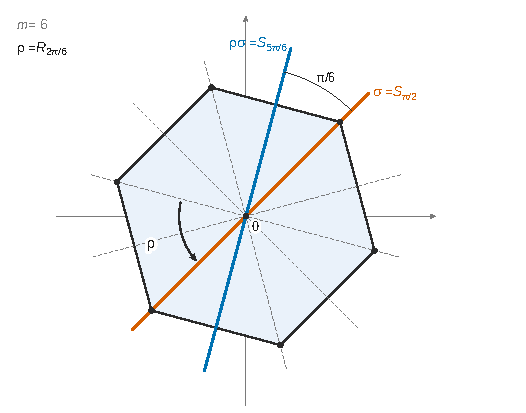
\includegraphics{figures/q8-groupe-diedral-hexagone.pdf}
\caption*{Figure 1 --- 𝒟₆ (m = 6) comme groupe des isométries d'un hexagone
régulier : 6 rotations ρᵏ et 6 symétries d'axes d'angles π/4 + kπ/6 ;
l'axe de ρσ se déduit de celui de σ par une rotation de π/6}
\end{figure}

\textbf{b)} Soit \(G\) fini avec \(G\not\subset{\mathrm{SO}}_2(\mathbb{R})\), et \(H=G\cap{\mathrm{SO}}_2(\mathbb{R})\).

C'est un sous-groupe fini de \({\mathrm{SO}}_2(\mathbb{R})\), donc \(H=\langle R_\alpha\rangle\) (Q7), de cardinal \(m\).

L'ordre de \(R_\alpha\) vaut \(m\), donc \(R_{m\alpha}=I_2\) et \(\alpha\in\frac{2\pi}{m}\mathbb{Z}\).

Ainsi \(H\subset\langle R_{2\pi/m}\rangle\), et ces groupes ont le même cardinal \(m\) : \(H=\mathcal{C}\).

Soit \(\tau\in G\setminus{\mathrm{SO}}_2(\mathbb{R})\). On a \(\det\tau=-1\) et, comme en Q4, \(\tau=S_\beta\) pour un \(\beta\in\mathbb{R}\) (première colonne \((\cos\beta,\sin\beta)\), seconde colonne unitaire orthogonale, signe fixé par le déterminant).

Le déterminant est un morphisme \(G\to\{\pm1\}\) de noyau \(H\).

Si \(\det g=-1\), alors \(g\tau\in H\) et \(g=(g\tau)\tau\). Donc \(G=H\sqcup H\tau\).

Posons \(\gamma=\frac{\beta-\pi/2}{2}\) et \(P=R_\gamma\). Alors

\equationajustee{\begin{aligned}P\sigma P^{-1}&=R_\gamma S_{\pi/2}R_{-\gamma}\\&=S_{\gamma+\pi/2}R_{-\gamma}\\&=S_{2\gamma+\pi/2}\\&=S_\beta=\tau,\end{aligned}}

et \(P\mathcal{C}P^{-1}=\mathcal{C}=H\) (commutativité de \({\mathrm{SO}}_2(\mathbb{R})\)). La conjugaison \(\Phi:M\mapsto PMP^{-1}\) est un morphisme injectif de \({\mathrm{GL}}_2(\mathbb{R})\), et

\equationajustee{\begin{aligned}\Phi({\mathcal{D}}_m)&=\Phi(\mathcal{C})\cup\Phi(\mathcal{C})\Phi(\sigma)\\&=H\cup H\tau\\&=G.\end{aligned}}

Donc

\equationajustee{\boxed{G\simeq{\mathcal{D}}_m\ \text{avec}\ m=|G\cap{\mathrm{SO}}_2(\mathbb{R})|=|G|/2\ \text{(et \text{même} \text{conjugué} dans }{\mathrm{O}}_2(\mathbb{R})).}}

\hypertarget{iii-une-caractuxe9risation-des-sous-groupes-finis-de-mathrmo_nmathbbr}{%
\subsection{\texorpdfstring{III --- Une caractérisation des sous-groupes finis de \({\mathrm{O}}_n(\mathbb{R})\)}{III --- Une caractérisation des sous-groupes finis de \{\textbackslash mathrm\{O\}\}\_n(\textbackslash mathbb\{R\})}}\label{iii-une-caractuxe9risation-des-sous-groupes-finis-de-mathrmo_nmathbbr}}

\hypertarget{q9}{%
\subsubsection{Q9}\label{q9}}

\textbf{Théorème.} Pour toute \(M\in{\mathrm{O}}_n(\mathbb{R})\), il existe \(P\in{\mathrm{O}}_n(\mathbb{R})\) telle que

\equationajustee{P^\top MP=\begin{pmatrix}I_p&&&&\\&-I_q&&&\\&&R_{\theta_1}&&\\&&&\ddots&\\&&&&R_{\theta_r}\end{pmatrix},}

avec \(p+q+2r=n\) et \(\theta_i\in\,]0,\pi[\) (ou \(\theta_i\in\mathbb{R}\setminus\pi\mathbb{Z}\)).

Version géométrique : toute isométrie d'un espace euclidien admet, dans une base orthonormée convenable, une matrice de cette forme. En particulier \(\operatorname{tr}M=p-q+2\sum_{i=1}^r\cos\theta_i\).

\hypertarget{q10}{%
\subsubsection{Q10}\label{q10}}

Soit \(m\in{\mathbb{N}}^*\) tel que \(M^m=I_n\) pour tout \(M\in G\). Soit \(M\in G\) ; avec les notations de Q9, la matrice \(D=P^\top MP\) vérifie

\equationajustee{D^m=P^\top M^mP=I_n.}

Par blocs, \(R_{\theta_i}^m=R_{m\theta_i}=I_2\), soit \(\theta_i\in\frac{2\pi}{m}\mathbb{Z}\), et \(\cos\theta_i\in C_m=\{\cos(2k\pi/m)\,;\,0\leqslant k<m\}\).

Par conséquent, \(\operatorname{tr}M\) appartient à l'ensemble \(T\) des réels

\equationajustee{p-q+2\sum_{i=1}^rc_i,}

où \(p+q+2r=n\) et \(c_1,\dots,c_r\in C_m\).

Cet ensemble est fini : au plus \((n+1)^2\) triplets \((p,q,r)\), et \(m^r\leqslant m^n\) choix des \(c_i\).

Comme \(\operatorname{tr}G\subset T\), \textbf{\(\operatorname{tr}G\) est fini.}

\hypertarget{q11}{%
\subsubsection{Q11}\label{q11}}

\(\mathcal{F}=\mathrm{Vect}(G)\) est de dimension finie \(d\leqslant n^2\). Les familles libres d'éléments de \(G\) ont au plus \(d\) éléments ; soit \((A_1,\dots,A_s)\) l'une d'elles, de cardinal maximal.

Soit \(M\in G\). Si \(M\notin\mathrm{Vect}(A_1,\dots,A_s)\), la famille \((A_1,\dots,A_s,M)\) serait libre et formée d'éléments de \(G\), ce qui contredit la maximalité.

Donc \(G\subset\mathrm{Vect}(A_i)\), puis \(\mathcal{F}=\mathrm{Vect}(A_1,\dots,A_s)\).

\textbf{\((A_1,\dots,A_s)\) est une base de \(\mathcal{F}\) formée d'éléments de \(G\), et \(s=d\).}

\hypertarget{q12}{%
\subsubsection{Q12}\label{q12}}

\textbf{a)} Chacune des \(d\) matrices \(A_i\) a \(n^2\) coordonnées : \(\boxed{C\in{\mathcal{M}}_{n^2,d}(\mathbb{R})}\) (la colonne \(i\) contient les coordonnées de \(A_i\)).

\textbf{b)} La base canonique est orthonormée :

\equationajustee{\begin{aligned}(E_{k\ell}|E_{k'\ell'})&=\operatorname{tr}(E_{\ell k}E_{k'\ell'})\\&=\delta_{kk'}\operatorname{tr}(E_{\ell\ell'})\\&=\delta_{kk'}\delta_{\ell\ell'}.\end{aligned}}

Par bilinéarité, en notant \(c_{\cdot i}\) la colonne \(i\) de \(C\),

\equationajustee{\begin{aligned}(A_i|A_j)&=\sum_{k=1}^{n^2}c_{ki}c_{kj}\\&=(C^\top C)_{ij},\end{aligned}}

donc

\equationajustee{\boxed{B=C^\top C.}}

\textbf{c)} Si \(CX=0\), alors \(C^\top CX=0\). Si \(C^\top CX=0\), alors

\equationajustee{0=X^\top C^\top CX=\|CX\|^2,}

donc \(CX=0\). Ainsi \(\ker B=\ker C\) et, par le théorème du rang (les deux matrices ont \(d\) colonnes), \(\operatorname{rg}B=\operatorname{rg}C\).

Les colonnes de \(C\) sont les coordonnées de la famille libre \((A_i)\), donc \(\operatorname{rg}C=d\). \textbf{\(B\in{\mathcal{M}}_d(\mathbb{R})\) est de rang \(d\), donc inversible.}

\hypertarget{q13}{%
\subsubsection{Q13}\label{q13}}

Pour \(i\in[\![1,d]\!]\), par linéarité,

\equationajustee{\begin{aligned}(A_i|M)&=\sum_{j=1}^d(A_i|A_j)x_j\\&=(BX_M)_i.\end{aligned}}

Donc \(Y_M=BX_M\) et, \(B\) étant inversible,

\equationajustee{\boxed{X_M=B^{-1}Y_M.}}

\hypertarget{q14}{%
\subsubsection{Q14}\label{q14}}

Soit \(M\in G\). Comme \(A_i\in G\subset{\mathrm{O}}_n(\mathbb{R})\), on a \(A_i^\top=A_i^{-1}\in G\), donc \(A_i^\top M\in G\) et

\equationajustee{(A_i|M)=\operatorname{tr}(A_i^\top M)\in\operatorname{tr}G.}

Ainsi \(\{Y_M\,;\,M\in G\}\subset(\operatorname{tr}G)^d\), qui est fini.

L'application \(M\mapsto Y_M\) est injective sur \(G\) : si \(Y_M=Y_{M'}\), alors \(X_M=X_{M'}\) (Q13), donc \(M=M'\). Une injection de \(G\) dans un ensemble fini donne

\equationajustee{\boxed{G\ \text{fini},\quad|G|\leqslant|\operatorname{tr}G|^d.}}

\emph{Bilan.} Pour \(G\subset{\mathrm{O}}_n(\mathbb{R})\) :

\begin{itemize}
\tightlist
\item
  Q1 : \(G\) fini \(\Rightarrow\) \(G\) d'exposant fini ;
\item
  Q10 : \(G\) d'exposant fini \(\Rightarrow\) \(\operatorname{tr}G\) fini ;
\item
  Q11--Q14 : \(\operatorname{tr}G\) fini \(\Rightarrow\) \(G\) fini.
\end{itemize}

Donc \(G\) fini \(\iff\) \(G\) d'exposant fini \(\iff\) \(\operatorname{tr}G\) fini.

\begin{center}\rule{0.5\linewidth}{0.5pt}\end{center}

\hypertarget{partie-b-sous-groupes-compacts-de-mathrmgl_nmathbbr}{%
\section{\texorpdfstring{Partie B --- Sous-groupes compacts de \({\mathrm{GL}}_n(\mathbb{R})\)}{Partie B --- Sous-groupes compacts de \{\textbackslash mathrm\{GL\}\}\_n(\textbackslash mathbb\{R\})}}\label{partie-b-sous-groupes-compacts-de-mathrmgl_nmathbbr}}

\hypertarget{i-quelques-propriuxe9tuxe9s-utiles}{%
\subsection{I --- Quelques propriétés utiles}\label{i-quelques-propriuxe9tuxe9s-utiles}}

\hypertarget{q15}{%
\subsubsection{Q15}\label{q15}}

On a

\equationajustee{\langle X,Y\rangle_A=(AX)^\top Y=X^\top AY,}

expression bilinéaire. Elle est symétrique car \(X^\top AY\) est un scalaire, égal à sa transposée \(Y^\top A^\top X=Y^\top AX\) (\(A\) symétrique).

Enfin \(\langle X,X\rangle_A=X^\top AX>0\) pour \(X\neq0\) (\(A\in{\mathcal{S}}_n^{++}(\mathbb{R})\)). \textbf{C'est un produit scalaire.}

Pour \(r>0\) et \(A=r^{-2}I_n\), on a \(\|X\|_A^2=\|X\|^2/r^2\), donc \({\mathcal{B}}_A=\{X\,;\,\|X\|\leqslant r\}=\mathcal{B}(0,r)\).

Pour \(r=0\), \(\mathcal{B}(0,0)=\{0\}\) n'est la boule unité d'aucune norme : elle contiendrait \(X/\|X\|_A\) pour \(X\ne0\). Donc

\equationajustee{\boxed{\mathcal{B}(0,r)={\mathcal{B}}_A\ \text{avec}\ A=r^{-2}I_n\ \text{si}\ r>0,}}

et \textbf{aucune matrice ne convient si \(r=0\).}

\hypertarget{q16}{%
\subsubsection{Q16}\label{q16}}

Soit \(u:X\mapsto A^{-1}BX\). Pour tous \(X,Y\) :

\equationajustee{\begin{aligned}\langle u(X),Y\rangle_A&=(AA^{-1}BX|Y)\\&=X^\top BY,\\\langle X,u(Y)\rangle_A&=X^\top A^\top A^{-1}BY\\&=X^\top BY,\end{aligned}}

en utilisant \(B^\top=B\) et \(A^\top=A\). \textbf{\(u\) est autoadjoint pour \(\langle\cdot,\cdot\rangle_A\).}

Par le théorème spectral dans l'espace euclidien \(({\mathcal{M}}_{n,1}(\mathbb{R}),\allowbreak \langle\cdot,\allowbreak \cdot\rangle_A)\), il existe une base \(\langle\cdot,\cdot\rangle_A\)-orthonormée \((\varepsilon_i)\) de vecteurs propres de \(u\) :

\equationajustee{\boxed{A^{-1}B\ \text{est diagonalisable sur}\ \mathbb{R}\ \text{(spectre \text{réel}), dans une base}\ \langle\cdot,\cdot\rangle_A\text{-\text{orthonormée}.}}}

(En général \(A^{-1}B\) n'est pas symétrique.)

\hypertarget{q17}{%
\subsubsection{Q17}\label{q17}}

\(A-B\) est symétrique et \(((A-B)X|X)=(AX|X)-(BX|X)\). Donc

\equationajustee{\begin{aligned}B\preccurlyeq A&\iff\forall X,\ ((A-B)X|X)\geqslant0\\&\iff\boxed{A-B\in{\mathcal{S}}_n^+(\mathbb{R})}.\end{aligned}}

\hypertarget{q18}{%
\subsubsection{Q18}\label{q18}}

Soit \(u:X\mapsto A^{-1}BX\) ; pour tous \(X,Y\), \((BX|Y)=\langle u(X),Y\rangle_A\).

\emph{Valeurs propres positives.} Si \(BX=\lambda AX\) avec \(X\neq0\), alors \((BX|X)=\lambda(AX|X)\) et \(\lambda=\frac{(BX|X)}{(AX|X)}>0\).

\emph{Sens direct.} Si \(B\preccurlyeq A\), ce même quotient est \(\leqslant1\) : \(\mathrm{Sp}(A^{-1}B)\subset\,]0,1]\).

\emph{Réciproque.} Soit \((\varepsilon_i)\) une base \(\langle\cdot,\cdot\rangle_A\)-orthonormée avec \(u(\varepsilon_i)=\lambda_i\varepsilon_i\) et \(\lambda_i\in\,]0,1]\) (Q16). Pour \(X=\sum x_i\varepsilon_i\) :

\equationajustee{\begin{aligned}(AX|X)&=\langle X,X\rangle_A\\&=\sum x_i^2,\\(BX|X)&=\langle u(X),X\rangle_A\\&=\sum\lambda_ix_i^2\\&\leqslant\sum x_i^2.\end{aligned}}

Donc \(B\preccurlyeq A\).

\equationajustee{\boxed{B\preccurlyeq A\iff\mathrm{Sp}(A^{-1}B)\subset\,]0,1].}}

\hypertarget{q19}{%
\subsubsection{Q19}\label{q19}}

\(\det A>0\) et, les valeurs propres \(\lambda_1,\dots,\lambda_n\) de \(A^{-1}B\) (diagonalisable) étant dans \(]0,1]\) (Q18),

\equationajustee{\begin{aligned}\frac{\det B}{\det A}&=\det(A^{-1}B)\\&=\prod_{i=1}^n\lambda_i\\&\leqslant1.\end{aligned}}

Supposons \(\det B=\det A\), c'est-à-dire \(\prod\lambda_i=1\) avec \(0<\lambda_i\leqslant1\).

Si un \(\lambda_{i_0}\) était \(<1\), le produit serait \(\leqslant\lambda_{i_0}<1\). Donc tous les \(\lambda_i\) valent \(1\).

La matrice \(A^{-1}B\), diagonalisable de seule valeur propre \(1\), vaut alors \(I_n\) : \(B=A\). La réciproque est claire.

\equationajustee{\boxed{\det B\leqslant\det A,\ \text{avec \text{égalité} si et seulement si}\ A=B.}}

\hypertarget{q20}{%
\subsubsection{Q20}\label{q20}}

On prend \(A,B\in{\mathcal{S}}_n^{++}(\mathbb{R})\) (pour que \({\mathcal{B}}_A,{\mathcal{B}}_B\) soient définies) ; \({\mathcal{B}}_A=\{X\,;\,(AX|X)\leqslant1\}\).

\((\Rightarrow)\) Si \(X\in{\mathcal{B}}_A\), \((BX|X)\leqslant(AX|X)\leqslant1\), donc \(X\in{\mathcal{B}}_B\).

\((\Leftarrow)\) Pour \(X=0\) l'inégalité est claire. Pour \(X\neq0\), posons \(t=(AX|X)^{-1/2}\) ; alors \((A(tX)|tX)=1\).

Donc \(tX\in{\mathcal{B}}_A\subset{\mathcal{B}}_B\) et \(t^2(BX|X)\leqslant1\), soit \((BX|X)\leqslant(AX|X)\).

\equationajustee{\boxed{B\preccurlyeq A\iff{\mathcal{B}}_A\subset{\mathcal{B}}_B.}}

\begin{figure}[H]
\centering
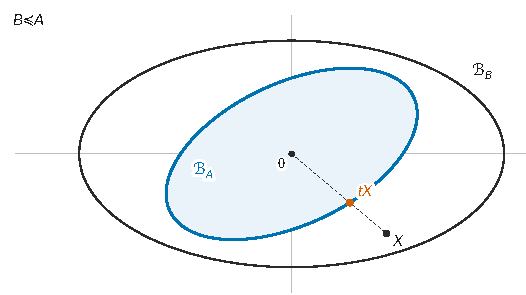
\includegraphics{figures/q20-inclusion-boules.pdf}
\caption*{Figure 2 --- B ≼ A équivaut à l'inclusion de la boule de A dans celle de
B (inclusion renversée) ; pour la réciproque, X est ramené en tX sur le
bord de la boule de A}
\end{figure}

\hypertarget{q21}{%
\subsubsection{Q21}\label{q21}}

Pour \(A\in{\mathcal{S}}_n^+(\mathbb{R})\) de valeurs propres \(\mu_1,\dots,\mu_n\geqslant0\) (base orthonormée propre \((e_i)\)), on a \(\|A\|^2=\operatorname{tr}(A^2)=\sum\mu_i^2\).

\((\Leftarrow)\) Supposons \(A\preccurlyeq\alpha I_n\) pour tout \(A\in\mathcal{K}\). Alors \(\mu_i=(Ae_i|e_i)\leqslant\alpha\), donc \(\mu_i\in[0,\alpha]\).

Ainsi \(\|A\|\leqslant\alpha\sqrt n\) : \(\mathcal{K}\) est bornée.

\((\Rightarrow)\) Supposons \(\|A\|\leqslant R\) (\(R>0\)) sur \(\mathcal{K}\). L'inégalité de Cauchy-Schwarz appliquée à chaque ligne donne \(\|AX\|\leqslant\|A\|\,\|X\|\), puis

\equationajustee{\begin{aligned}(AX|X)&\leqslant\|AX\|\,\|X\|\\&\leqslant R\|X\|^2\\&=(RI_nX|X).\end{aligned}}

Donc \(A\preccurlyeq RI_n\).

\equationajustee{\boxed{\mathcal{K}\ \text{\text{bornée}}\iff\exists\alpha>0,\ \forall A\in\mathcal{K},\ A\preccurlyeq\alpha I_n.}}

\hypertarget{ii-stricte-log-concavituxe9-de-lapplication-det}{%
\subsection{\texorpdfstring{II --- Stricte log-concavité de l'application \(\det\)}{II --- Stricte log-concavité de l'application \textbackslash det}}\label{ii-stricte-log-concavituxe9-de-lapplication-det}}

\hypertarget{q22}{%
\subsubsection{Q22}\label{q22}}

Soient \(A,B\in{\mathcal{S}}_n^{++}(\mathbb{R})\) et \(t\in[0,1]\). La matrice \(M=tA+(1-t)B\) est symétrique et, pour \(X\neq0\),

\equationajustee{(MX|X)=t(AX|X)+(1-t)(BX|X)>0,}

car les deux termes \((AX|X)\) et \((BX|X)\) sont \(>0\), et \(t,1-t\geqslant0\) ne sont pas tous deux nuls. \textbf{\({\mathcal{S}}_n^{++}(\mathbb{R})\) est convexe.}

\hypertarget{q23}{%
\subsubsection{Q23}\label{q23}}

Soient \(A,B\in{\mathcal{S}}_n^{++}(\mathbb{R})\). Pour \(t\in\{0,1\}\) il y a égalité ; soit \(t\in\,]0,1[\).

\emph{Réduction simultanée.} Par Q16 et Q18, il existe une base \((\varepsilon_i)\), \(\langle\cdot,\cdot\rangle_A\)-orthonormée, avec \(A^{-1}B\varepsilon_i=\lambda_i\varepsilon_i\) et \(\lambda_i>0\).

Soit \(P\) la matrice (inversible) de colonnes \(\varepsilon_i\). Alors

\equationajustee{\begin{aligned}(P^\top AP)_{ij}&=\langle\varepsilon_i,\varepsilon_j\rangle_A\\&=\delta_{ij},\\(P^\top BP)_{ij}&=\langle\varepsilon_i,u(\varepsilon_j)\rangle_A\\&=\lambda_j\delta_{ij}.\end{aligned}}

Donc \(P^\top AP=I_n\) et \(P^\top BP=D=\mathrm{diag}(\lambda_i)\).

\emph{Déterminants.} Posons \(c=(\det P)^2>0\). Alors

\equationajustee{\begin{aligned}c\det A&=1,\\c\det B&=\prod\lambda_i,\\c\det(tA+(1-t)B)&=\prod(t+(1-t)\lambda_i).\end{aligned}}

Donc

\equationajustee{\varphi(tA+(1-t)B)-t\varphi(A)-(1-t)\varphi(B)=\sum_{i=1}^n\Bigl[\ln\bigl(t+(1-t)\lambda_i\bigr)-(1-t)\ln\lambda_i\Bigr].}

\emph{Inégalité scalaire.} Pour \(\lambda>0\), soit \(g(\lambda)=t+(1-t)\lambda-\lambda^{1-t}\). Alors

\equationajustee{g'(\lambda)=(1-t)(1-\lambda^{-t}),}

qui est \(<0\) sur \(]0,1[\) et \(>0\) sur \(]1,+\infty[\).

Donc \(g\geqslant g(1)=0\), avec égalité si et seulement si \(\lambda=1\). Ainsi

\equationajustee{\ln(t+(1-t)\lambda)\geqslant(1-t)\ln\lambda,}

avec égalité si et seulement si \(\lambda=1\).

\emph{Conclusion.} Chaque crochet est \(\geqslant0\), donc

\equationajustee{\varphi(tA+(1-t)B)\geqslant t\varphi(A)+(1-t)\varphi(B).}

Il y a égalité si et seulement si tous les \(\lambda_i\) valent \(1\), c'est-à-dire \(D=I_n\), soit \(P^\top BP=P^\top AP\), soit \(B=A\).

\equationajustee{\boxed{\varphi=\ln\circ\det\ \text{est strictement concave sur}\ {\mathcal{S}}_n^{++}(\mathbb{R}).}}

\hypertarget{iii-groupe-orthogonal-associuxe9-uxe0-une-matrice-symuxe9trique-duxe9finie-positive}{%
\subsection{III --- Groupe orthogonal associé à une matrice symétrique définie positive}\label{iii-groupe-orthogonal-associuxe9-uxe0-une-matrice-symuxe9trique-duxe9finie-positive}}

\hypertarget{q24}{%
\subsubsection{Q24}\label{q24}}

\emph{Existence de \(B\).} Par le théorème spectral, \(A=Q\Delta Q^\top\) avec \(Q\in{\mathrm{O}}_n(\mathbb{R})\) et \(\Delta=\mathrm{diag}(\mu_i)\), \(\mu_i>0\).

Avec \(B=\Delta^{1/2}Q^\top\) (inversible), on a \(B^\top B=Q\Delta Q^\top=A\).

\emph{Sous-groupe.} Si \(M^\top AM=A\), alors \((\det M)^2\det A=\det A\neq0\), donc \(\det M=\pm1\) : \(\mathrm{O}(A)\subset{\mathrm{GL}}_n(\mathbb{R})\).

Ensuite \(I_n\in\mathrm{O}(A)\) et, pour \(M,N\in\mathrm{O}(A)\),

\equationajustee{\begin{aligned}(MN)^\top A(MN)&=N^\top(M^\top AM)N\\&=A,\\(M^{-1})^\top AM^{-1}&=(M^{-1})^\top(M^\top AM)M^{-1}\\&=A.\end{aligned}}

\emph{Isomorphisme.} \(\Psi:N\mapsto B^{-1}NB\) est un morphisme injectif de \({\mathrm{GL}}_n(\mathbb{R})\) dans lui-même. Avec \(M=B^{-1}NB\) :

\equationajustee{M^\top AM=B^\top N^\top(B^{-1})^\top B^\top BB^{-1}NB=B^\top N^\top NB,}

donc \(M^\top AM=A=B^\top B\iff N^\top N=I_n\) (\(B\) inversible). Ainsi \(\Psi({\mathrm{O}}_n(\mathbb{R}))=\mathrm{O}(A)\) :

\equationajustee{\boxed{\Psi:N\mapsto B^{-1}NB\ \text{est un isomorphisme de}\ {\mathrm{O}}_n(\mathbb{R})\ \text{sur}\ \mathrm{O}(A).}}

\hypertarget{q25}{%
\subsubsection{Q25}\label{q25}}

\({\mathrm{O}}_n(\mathbb{R})=f^{-1}(\{I_n\})\), avec \(f:M\mapsto M^\top M\) continue : il est fermé. Il est borné car \(\|M\|^2=\operatorname{tr}(M^\top M)=n\). En dimension finie, il est donc compact.

\(\Psi\) est linéaire donc continue, et \(\mathrm{O}(A)=\Psi({\mathrm{O}}_n(\mathbb{R}))\) (Q24) : \textbf{\(\mathrm{O}(A)\) est compact}, comme image continue d'un compact.

\hypertarget{iv-sous-groupes-compacts-de-mathrmgl_nmathbbr}{%
\subsection{\texorpdfstring{IV --- Sous-groupes compacts de \({\mathrm{GL}}_n(\mathbb{R})\)}{IV --- Sous-groupes compacts de \{\textbackslash mathrm\{GL\}\}\_n(\textbackslash mathbb\{R\})}}\label{iv-sous-groupes-compacts-de-mathrmgl_nmathbbr}}

\hypertarget{q26}{%
\subsubsection{Q26}\label{q26}}

Soit \(M\in G\) et \(a=|\det M|>0\). Pour \(k\in\mathbb{Z}\), \(M^k\in G\) et \(|\det M^k|=a^k\).

L'application continue \(M\mapsto|\det M|\) est bornée sur le compact \(G\), donc la suite \((a^k)_{k\in\mathbb{Z}}\) est bornée.

Or, si \(a>1\), \(a^k\to+\infty\) quand \(k\to+\infty\).

Si \(a<1\), \(a^k\to+\infty\) quand \(k\to-\infty\). Donc

\equationajustee{\boxed{\forall M\in G,\ |\det M|=1.}}

\hypertarget{q27}{%
\subsubsection{Q27}\label{q27}}

\(\mathcal{B}\) est fermée bornée en dimension finie, donc compacte ; \(G\times\mathcal{B}\) est compact (produit de compacts).

L'application \(\Theta:(M,X)\mapsto MX\) est continue (coordonnées polynomiales). Donc \(\mathcal{C}=\Theta(G\times\mathcal{B})\) \textbf{est compact.}

Comme \(I_n\in G\), on a \(\mathcal{B}\subset\mathcal{C}\).

Donc \(\mathcal{C}\) contient la boule ouverte de centre \(0\) et de rayon \(1\) : \textbf{\(0\) est intérieur à \(\mathcal{C}\).}

\hypertarget{q28}{%
\subsubsection{Q28}\label{q28}}

Pour \(A\in{\mathcal{S}}_n^+(\mathbb{R})\), on pose \({\mathcal{B}}_A=\{X\,;\,(AX|X)\leqslant1\}\) (ce qui prolonge la définition de la partie I), et \(\mathcal{E}=\{A\in{\mathcal{S}}_n^+(\mathbb{R})\,;\,\mathcal{C}\subset{\mathcal{B}}_A\}\).

\emph{Non vide.} \(\mathcal{C}\) est borné : \(\mathcal{C}\subset\mathcal{B}(0,R)\) avec \(R>0\).

Par Q15, \(\mathcal{B}(0,R)={\mathcal{B}}_{A_0}\) avec \(A_0=R^{-2}I_n\), donc \(A_0\in\mathcal{E}\).

\emph{Convexe.} Soient \(A,A'\in\mathcal{E}\) et \(t\in[0,1]\). On a \(tA+(1-t)A'\in{\mathcal{S}}_n^+(\mathbb{R})\) (calcul de Q22 avec des inégalités larges).

Pour \(X\in\mathcal{C}\), \(((tA+(1-t)A')X|X)\leqslant t+(1-t)=1\).

\emph{Fermé.} \({\mathcal{S}}_n(\mathbb{R})\) est un sous-espace, donc fermé, et pour \(X\) fixé \(A\mapsto(AX|X)\) est linéaire, donc continue. Ainsi

\equationajustee{\mathcal{E}=\bigcap_{X\in{\mathcal{M}}_{n,1}(\mathbb{R})}\{A\in{\mathcal{S}}_n(\mathbb{R})\,;\,(AX|X)\geqslant0\}\ \cap\ \bigcap_{X\in\mathcal{C}}\{A\in{\mathcal{S}}_n(\mathbb{R})\,;\,(AX|X)\leqslant1\}}

est une intersection de fermés.

\emph{Borné.} On a \(\mathcal{B}\subset\mathcal{C}\) (Q27). Soit \(A\in\mathcal{E}\) et \(Y\neq0\) ; alors \(X=Y/\|Y\|\in\mathcal{C}\), donc \((AX|X)\leqslant1\).

Ainsi \((AY|Y)\leqslant\|Y\|^2\), c'est-à-dire \(A\preccurlyeq I_n\). Par Q21, \(\mathcal{E}\) est bornée.

Fermé borné en dimension finie, \textbf{\(\mathcal{E}\) est compact, non vide et convexe.}

\emph{Existence.} \(\det\) est continue ; elle atteint son maximum sur \(\mathcal{E}\) en un point \(A_1\), et \(\det A_1\geqslant\det A_0=R^{-2n}>0\).

Les valeurs propres de \(A_1\in{\mathcal{S}}_n^+(\mathbb{R})\) sont \(\geqslant0\) et de produit non nul, donc \(A_1\in{\mathcal{S}}_n^{++}(\mathbb{R})\).

\emph{Unicité.} Soient \(A_1\neq A_2\) deux points de \(\mathcal{E}\) où \(\det\) vaut son maximum \(m>0\) ; ils sont dans \({\mathcal{S}}_n^{++}(\mathbb{R})\).

La matrice \(A_3=\frac12(A_1+A_2)\) appartient à \(\mathcal{E}\cap{\mathcal{S}}_n^{++}(\mathbb{R})\) et, par Q23 avec \(t=\frac12\) et \(A_1\neq A_2\),

\equationajustee{\begin{aligned}\ln\det A_3&>\tfrac12\ln m+\tfrac12\ln m\\&=\ln m,\end{aligned}}

ce qui contredit la maximalité. Donc \(A_1=A_2\).

Toute \(A\in{\mathcal{S}}_n^{++}(\mathbb{R})\) telle que \(\mathcal{C}\subset{\mathcal{B}}_A\) est dans \(\mathcal{E}\), donc

\equationajustee{\boxed{\text{il existe une unique}\ A\in{\mathcal{S}}_n^{++}(\mathbb{R})\ \text{telle que}\ \mathcal{C}\subset{\mathcal{B}}_A\ \text{et}\ \det A\ \text{maximal.}}}

\begin{figure}[H]
\centering
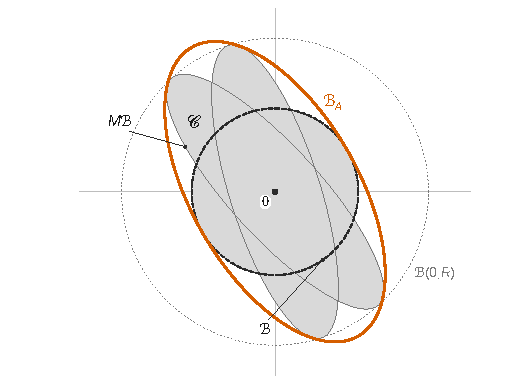
\includegraphics{figures/q28-ellipse-determinant-maximal.pdf}
\caption*{Figure 3 --- 𝒞, réunion des ellipses Mℬ (M ∈ G), contient ℬ ; parmi les
ellipses centrées en 0 qui contiennent 𝒞, dont ℬ(0, R), celle de
déterminant maximal est unique}
\end{figure}

\hypertarget{q29}{%
\subsubsection{Q29}\label{q29}}

Soit \(A\) la matrice de Q28, \(M\in G\) et \(A'=M^\top AM\).

\begin{itemize}
\tightlist
\item
  \(A'\in{\mathcal{S}}_n^{++}(\mathbb{R})\) : elle est symétrique et \((A'X|X)=(AMX|MX)>0\) pour \(X\neq0\), car \(M\) est inversible.
\item
  \(\det A'=(\det M)^2\det A=\det A\) (Q26).
\item
  \(\mathcal{C}\subset{\mathcal{B}}_{A'}\) : voir ci-dessous.
\end{itemize}

Soit en effet \(Y=NX\in\mathcal{C}\), avec \(N\in G\) et \(X\in\mathcal{B}\).

Comme \(MN\in G\), on a \(MY=(MN)X\in\mathcal{C}\subset{\mathcal{B}}_A\), donc \((A'Y|Y)=(AMY|MY)\leqslant1\).

\(A'\) est donc admissible et de déterminant maximal ; par unicité (Q28), \(A'=A\), soit \(M^\top AM=A\) et \(M\in\mathrm{O}(A)\). Comme \(G\) est un groupe pour la même loi,

\equationajustee{\boxed{G\ \text{est un sous-groupe de}\ \mathrm{O}(A).}}

Par Q24, \(\Psi^{-1}(G)=BGB^{-1}\) est un sous-groupe de \({\mathrm{O}}_n(\mathbb{R})\) isomorphe à \(G\) : tout sous-groupe compact de \({\mathrm{GL}}_n(\mathbb{R})\) est conjugué à un sous-groupe de \({\mathrm{O}}_n(\mathbb{R})\).

\begin{center}\rule{0.5\linewidth}{0.5pt}\end{center}

\hypertarget{partie-c-croissance-du-groupe-de-heisenberg-discret}{%
\section{Partie C --- Croissance du groupe de Heisenberg discret}\label{partie-c-croissance-du-groupe-de-heisenberg-discret}}

Dans la définition de \(\ell_{\mathcal{S}}\), les \(s_i\) parcourent \(\mathcal{S}\) avec répétitions possibles et \(k\) est quelconque.

Ainsi \(\ell_{\mathcal{S}}(g)\) est la longueur minimale d'un mot en les \(s^{\pm1}\), \(s\in\mathcal{S}\), représentant \(g\).

\hypertarget{i-croissance-dun-groupe}{%
\subsection{I --- Croissance d'un groupe}\label{i-croissance-dun-groupe}}

\hypertarget{q30}{%
\subsubsection{Q30}\label{q30}}

Comme \(\mathcal{S}\) engendre \(G\), tout \(g\) admet une écriture \(s_1^{a_1}\cdots s_k^{a_k}\).

L'ensemble des poids \(\sum|a_i|\) est une partie non vide de \(\mathbb{N}\) : \(\ell_{\mathcal{S}}(g)\) est bien défini.

\emph{Inverse.} Soit \(g=s_1^{a_1}\cdots s_k^{a_k}\) une écriture de poids \(\ell_{\mathcal{S}}(g)\). Alors \(g^{-1}=s_k^{-a_k}\cdots s_1^{-a_1}\) a le même poids, donc \(\ell_{\mathcal{S}}(g^{-1})\leqslant\ell_{\mathcal{S}}(g)\).

Appliqué à \(g^{-1}\), cela donne l'inégalité inverse. (Pour \(g=e\) : \(0=0\).)

\emph{Produit.} Concaténons des écritures minimales de \(g\) et \(h\) (vides si \(g=e\) ou \(h=e\)).

On obtient une écriture de \(gh\) de poids \(\ell_{\mathcal{S}}(g)+\ell_{\mathcal{S}}(h)\). Donc

\equationajustee{\boxed{\begin{aligned}\ell_{\mathcal{S}}(g^{-1})&=\ell_{\mathcal{S}}(g),\\\ell_{\mathcal{S}}(gh)&\leqslant\ell_{\mathcal{S}}(g)+\ell_{\mathcal{S}}(h).\end{aligned}}}

\hypertarget{q31}{%
\subsubsection{Q31}\label{q31}}

Posons \(C'=\max(1,\max_{s\in\mathcal{S}}\ell_\Sigma(s))\) et \(D=\max(1,\max_{\sigma\in\Sigma}\ell_{\mathcal{S}}(\sigma))\), entiers \(\geqslant1\).

Par Q30, \(\ell_\Sigma(s^a)\leqslant|a|\,\ell_\Sigma(s)\leqslant|a|C'\). Pour une écriture minimale \(g=s_1^{a_1}\cdots s_k^{a_k}\) :

\equationajustee{\begin{aligned}\ell_\Sigma(g)&\leqslant\sum_i\ell_\Sigma(s_i^{a_i})\\&\leqslant C'\sum_i|a_i|\\&=C'\ell_{\mathcal{S}}(g).\end{aligned}}

Symétriquement \(\ell_{\mathcal{S}}(g)\leqslant D\,\ell_\Sigma(g)\). Avec \(C=1/D\) :

\equationajustee{\boxed{\forall g\in G,\quad C\,\ell_{\mathcal{S}}(g)\leqslant\ell_\Sigma(g)\leqslant C'\,\ell_{\mathcal{S}}(g).}}

\emph{Conséquence.} Supposons \(\alpha p^d\leqslant|{\mathcal{V}}_{\mathcal{S}}(p)|\leqslant\beta p^d\) pour \(p\geqslant1\).

\begin{itemize}
\tightlist
\item
  Si \(\ell_\Sigma(g)\leqslant p\), alors \(\ell_{\mathcal{S}}(g)\leqslant Dp\) : \({\mathcal{V}}_\Sigma(p)\subset{\mathcal{V}}_{\mathcal{S}}(Dp)\) et \(|{\mathcal{V}}_\Sigma(p)|\leqslant\beta D^dp^d\).
\item
  Si \(\ell_{\mathcal{S}}(g)\leqslant q:=\lfloor p/C'\rfloor\), alors \(\ell_\Sigma(g)\leqslant C'q\leqslant p\) : \({\mathcal{V}}_{\mathcal{S}}(q)\subset{\mathcal{V}}_\Sigma(p)\).
\end{itemize}

Pour \(p\geqslant C'\), on a \(q\geqslant1\) et \(q\geqslant\frac{p}{2C'}\), car \(\lfloor x\rfloor\geqslant x/2\) pour \(x\geqslant1\). D'où

\equationajustee{|{\mathcal{V}}_\Sigma(p)|\geqslant\alpha(2C')^{-d}p^d.}

Pour \(1\leqslant p<C'\), \(|{\mathcal{V}}_\Sigma(p)|\geqslant1\geqslant(p/C')^d\).

Avec \(\alpha'=\min(\alpha(2C')^{-d},C'^{-d})\) et \(\beta'=\beta D^d\), on a donc, pour tout \(p\geqslant1\),

\equationajustee{\alpha'p^d\leqslant|{\mathcal{V}}_\Sigma(p)|\leqslant\beta'p^d.}

\textbf{La croissance polynomiale de degré \(d\) ne dépend pas de la partie génératrice finie.}

\hypertarget{q32}{%
\subsubsection{Q32}\label{q32}}

Le nombre de \((x,y,z)\in{\mathbb{N}}^3\) avec \(x+y+z=s\) vaut \(\sum_{x=0}^s(s-x+1)=\binom{s+2}{2}\).

Par la formule de Pascal \(\binom{s+2}{2}=\binom{s+3}{3}-\binom{s+2}{3}\), la somme télescope. Le nombre

\equationajustee{N(p)=\#\{(x,y,z)\in{\mathbb{N}}^3\,;\,x+y+z\leqslant p\}}

vérifie

\equationajustee{\begin{aligned}N(p)&=\sum_{s=0}^p\binom{s+2}{2}\\&=\binom{p+3}{3}\\&=\boxed{\frac{(p+1)(p+2)(p+3)}{6}}.\end{aligned}}

Pour \(\mathcal{S}=\{e_1,e_2,e_3\}\) dans \(({\mathbb{Z}}^3,+)\), l'écriture \(xe_1+ye_2+ze_3\) donne \(\ell_{\mathcal{S}}(x,y,z)\leqslant|x|+|y|+|z|\).

Inversement, dans toute écriture \(\sum a_ie_{j_i}\), \(x\) est la somme des \(a_i\) avec \(j_i=1\), et de même pour \(y\) et \(z\).

Donc \(|x|+|y|+|z|\leqslant\sum|a_i|\). Ainsi \(\ell_{\mathcal{S}}(x,y,z)=|x|+|y|+|z|\) et

\equationajustee{{\mathcal{V}}_{\mathcal{S}}(p)=\{|x|+|y|+|z|\leqslant p\}.}

Cet ensemble contient les triplets de \({\mathbb{N}}^3\) de somme \(\leqslant p\), et \((x,y,z)\mapsto(|x|,|y|,|z|)\) l'envoie sur ces triplets avec des fibres d'au plus \(8\) éléments. Pour \(p\geqslant1\) :

\equationajustee{\begin{aligned}\frac{p^3}{6}\leqslant N(p)&\leqslant|{\mathcal{V}}_{\mathcal{S}}(p)|\\&\leqslant8N(p)\\&\leqslant\frac{8\cdot2p\cdot3p\cdot4p}{6}\\&=32p^3.\end{aligned}}

\equationajustee{\boxed{({\mathbb{Z}}^3,+)\ \text{est \text{à} croissance polynomiale de \text{degré}}\ 3.}}

(Valeur exacte : \(|{\mathcal{V}}_{\mathcal{S}}(p)|=\frac{(2p+1)(2p^2+2p+3)}{3}\), soit \(7,25,63,\dots\))

\hypertarget{ii-le-groupe-de-heisenberg-discret}{%
\subsection{II --- Le groupe de Heisenberg discret}\label{ii-le-groupe-de-heisenberg-discret}}

On note \(M(i,j,k)=\begin{pmatrix}1&j&k\\0&1&i\\0&0&1\end{pmatrix}\).

\hypertarget{q33}{%
\subsubsection{Q33}\label{q33}}

On a \(S=I_3+E_{23}\), \(T=I_3+E_{12}\) et \(U=I_3+E_{13}\), et \(E^2=0\) pour ces trois matrices \(E\).

D'où \((I_3+E)^m=I_3+mE\) pour \(m\in\mathbb{N}\), puis pour \(m\in\mathbb{Z}\) car \((I_3+E)^{-1}=I_3-E\).

Comme les produits \(E_{23}E_{12}\), \(E_{12}E_{13}\) et \(E_{23}E_{13}\) sont nuls,

\equationajustee{\boxed{\begin{aligned}S^iT^jU^k&=I_3+iE_{23}+jE_{12}+kE_{13}\\&=\begin{pmatrix}1&j&k\\0&1&i\\0&0&1\end{pmatrix}\\&=M(i,j,k).\end{aligned}}}

\hypertarget{q34}{%
\subsubsection{Q34}\label{q34}}

Par produit matriciel,

\equationajustee{M(i,j,k)M(i',j',k')=\begin{pmatrix}1&j+j'&k+k'+ji'\\0&1&i+i'\\0&0&1\end{pmatrix},}

donc

\equationajustee{\boxed{(i'',j'',k'')=(i+i',\ j+j',\ k+k'+ji').}}

Conséquence : \(K=\{M(i,j,k)\}\) est stable par produit, contient \(I_3\), et \(M(i,j,k)^{-1}=M(-i,-j,ij-k)\).

C'est un sous-groupe contenant \(S,T,U\), donc \(\mathbb{H}\subset K\), et \(K\subset\mathbb{H}\) par Q33. Ainsi \(\mathbb{H}=\{M(i,j,k)\,;\,(i,j,k)\in{\mathbb{Z}}^3\}\).

\hypertarget{q35}{%
\subsubsection{Q35}\label{q35}}

Par Q34, \(M(i,j,k)U=M(i,j,k+1)=UM(i,j,k)\) : \textbf{\(U\) commute avec tout élément de \(\mathbb{H}\).} Et

\equationajustee{\begin{aligned}T^jS^i&=M(0,j,0)M(i,0,0)\\&=M(i,j,ij)\\&=S^iT^jU^{ij},\end{aligned}}

donc

\equationajustee{\boxed{S^iT^jU^{ij}=T^jS^i.}}

\hypertarget{q36}{%
\subsubsection{Q36}\label{q36}}

\(ST=M(1,1,0)\neq M(1,1,1)=TS\) : \textbf{\(\mathbb{H}\) n'est pas commutatif.}

Avec \(i=j=1\), Q35 donne \(STU=TS\), donc \(U=T^{-1}S^{-1}TS\in\langle S,T\rangle\). Ainsi \(\langle S,T\rangle\) contient \(S,T,U\) :

\equationajustee{\boxed{\langle S,T\rangle=\mathbb{H}.}}

\hypertarget{q37}{%
\subsubsection{Q37}\label{q37}}

On a \(f(i,j,k)=S^iT^jU^k\in\mathbb{H}\) : \(f\) est bien définie.

Par Q33 et Q34, \(f(i,j,k)=M(i,j,k)\) et tout élément de \(\mathbb{H}\) est de cette forme : \(f\) est surjective.

Elle est injective : les coefficients d'indices \((2,3)\), \((1,2)\), \((1,3)\) de \(M(i,j,k)\) forment le triplet \((i,j,k)\).

\(f\) \textbf{n'est pas un morphisme} pour \(({\mathbb{Z}}^3,+)\) : sinon \(\mathbb{H}=f({\mathbb{Z}}^3)\) serait commutatif ; concrètement \(f((0,1,0)+(1,0,0))=ST\neq TS=f(0,1,0)f(1,0,0)\).

\textbf{Oui} : par transport de structure, la loi

\equationajustee{\begin{aligned}(i,j,k)*(i',j',k')&=f^{-1}\bigl(f(i,j,k)f(i',j',k')\bigr)\\&=(i+i',\ j+j',\ k+k'+ji')\end{aligned}}

est une loi de groupe sur \({\mathbb{Z}}^3\) (associativité héritée de \(\mathbb{H}\), neutre \((0,0,0)\), symétrique \((-i,-j,ij-k)\)), et \(f:({\mathbb{Z}}^3,*)\to\mathbb{H}\) est un isomorphisme.

\hypertarget{q38}{%
\subsubsection{Q38}\label{q38}}

\emph{Lemme.} Par récurrence à partir de Q34,

\equationajustee{\prod_{\ell=1}^rM(i_\ell,j_\ell,k_\ell)=M\Bigl(\sum_\ell i_\ell,\ \sum_\ell j_\ell,\ \sum_\ell k_\ell+\sum_{\ell<\ell'}j_\ell i_{\ell'}\Bigr)}

(au rang \(r+1\), le nouveau terme croisé est \(\bigl(\sum_{\ell\leqslant r}j_\ell\bigr)i_{r+1}\)).

\emph{Forme normale.} Soit \(M\in\mathbb{H}\) avec \(\ell_{\mathcal{A}}(M)\leqslant p\), et \(M=X_1^{a_1}\cdots X_r^{a_r}\) une écriture minimale.

Chaque facteur est \(M(a_\ell,0,0)\), \(M(0,a_\ell,0)\) ou \(M(0,0,a_\ell)\) ; notons \(i_\ell,j_\ell,k_\ell\) ses trois paramètres (deux sont nuls).

Le lemme donne \(M=S^iT^jU^{k+z}\), avec

\equationajustee{\begin{aligned}i&=\sum_\ell i_\ell,\\j&=\sum_\ell j_\ell,\\k&=\sum_\ell k_\ell,\\z&=\sum_{\ell<\ell'}j_\ell i_{\ell'}.\end{aligned}}

Alors \(|i|+|j|+|k|\leqslant\sum|a_\ell|\leqslant p\). Posons \(\hat\imath=\sum|i_\ell|\) et \(\hat\jmath=\sum|j_\ell|\), de sorte que \(\hat\imath+\hat\jmath\leqslant p\). Alors

\equationajustee{\begin{aligned}|z|&\leqslant\hat\imath\,\hat\jmath\\&\leqslant\Bigl(\frac{\hat\imath+\hat\jmath}{2}\Bigr)^2\\&\leqslant\frac{p^2}{4}.\end{aligned}}

\equationajustee{\boxed{\begin{aligned}{}&M=S^iT^jU^{k+z},\\&|i|+|j|+|k|\leqslant p,\\&|z|\leqslant\hat\imath\hat\jmath\leqslant p^2/4.\end{aligned}}}

\emph{La borne \(|z|\leqslant|ij|\) de l'énoncé est fausse en général.} On l'obtient quand les blocs \(S\) ont tous des exposants de même signe, ainsi que les blocs \(T\) (\(\hat\imath=|i|\), \(\hat\jmath=|j|\)).

Mais \(ST^3S^{-1}=M(0,3,-3)\) (lemme) a une longueur \(\leqslant5\).

Comme \(f\) est bijective, toute écriture \(M(0,3,-3)=S^iT^jU^{k+z}\) impose \(i=0\) et \(j=3\), donc \(|ij|=0\).

Alors \(z=0\), \(k=-3\) et \(|i|+|j|+|k|=6>5\).

De même, \(S^{10}T^{10}S^{-10}=M(0,10,-100)\) est de longueur \(\leqslant30\).

La majoration \(|z|\leqslant p^2/4\) remplace celle de l'énoncé et suffit pour la suite.

\emph{Dénombrement.} Soit \(M\in{\mathcal{V}}_{\mathcal{A}}(p)\). Alors \(M=M(i,j,m)\) avec \(|i|\leqslant p\), \(|j|\leqslant p\) et \(|m|\leqslant|k|+|z|\leqslant p+p^2/4\).

Comme \(f\) est injective, pour \(p\geqslant1\),

\equationajustee{\begin{aligned}|{\mathcal{V}}_{\mathcal{A}}(p)|&\leqslant(2p+1)^2\Bigl(2p+\frac{p^2}{2}+1\Bigr)\\&\leqslant9p^2\cdot\frac72p^2\\&\leqslant32p^4.\end{aligned}}

\equationajustee{\boxed{|{\mathcal{V}}_{\mathcal{A}}(p)|=O(p^4),\ \text{et \text{même}}\ |{\mathcal{V}}_{\mathcal{A}}(p)|\leqslant32p^4\ \text{pour}\ p\geqslant1.}}

\hypertarget{q39}{%
\subsubsection{Q39}\label{q39}}

\emph{Cas \(i,j,k\in\mathbb{N}\), \(i+j\leqslant p\), \(k\leqslant ij\).}

Si \(j=0\), alors \(k=0\) et \(S^i\) a un poids \(i\leqslant p\).

Si \(j\geqslant1\), écrivons \(k=jq+r\) avec \(0\leqslant r<j\) ; alors \(q\leqslant i\).

Si \(q<i\), on pose \((u,v)=(q+1,q)\).

Si \(q=i\), alors \(r=0\) et \(k=ij\) ; on pose \((u,v)=(i,i)\).

Avec \(a=i-u\), \(b=u-v\) et \(c=v\), entiers naturels de somme \(i\), le mot

\equationajustee{W=S^aT^rS^bT^{j-r}S^c}

a pour poids \(i+j\leqslant p\), et le lemme de Q38 donne \(W=M(i,j,z)\) avec

\equationajustee{\begin{aligned}z&=r(b+c)+(j-r)c\\&=ru+(j-r)v.\end{aligned}}

Si \(q<i\) : \(z=r(q+1)+(j-r)q=k\). Si \(q=i\) : \(z=ji=k\).

Donc \(W=S^iT^jU^k\) et \(\ell_{\mathcal{A}}(S^iT^jU^k)\leqslant i+j\leqslant p\).

\emph{Cas \(k\) du signe de \(ij\).} Les applications \(\psi_1:M(i,j,k)\mapsto M(-i,j,-k)\) et \(\psi_2:M(i,j,k)\mapsto M(i,-j,-k)\) sont des morphismes involutifs de \(\mathbb{H}\) (vérification directe sur la formule de Q34).

Ils envoient \(\{S^{\pm1},T^{\pm1},U^{\pm1}\}\) dans lui-même, donc conservent \(\ell_{\mathcal{A}}\).

Supposons \(|i|+|j|\leqslant p\), \(|k|\leqslant|ij|\) et \(k\,ij\geqslant0\).

Par \(\psi_1\) et \(\psi_2\), on se ramène à \(i,j\geqslant0\), donc à \(k\geqslant0\) (et \(k=0\) si \(ij=0\)), et le premier cas s'applique :

\equationajustee{\boxed{|i|+|j|\leqslant p,\ |k|\leqslant|ij|,\ k\,ij\geqslant0\ \Longrightarrow\ \ell_{\mathcal{A}}(S^iT^jU^k)\leqslant p.}}

\emph{Sans la condition de signe, l'énoncé est faux.} Prenons \((i,j,k)=(1,1,-1)\) et \(p=2\).

Par le lemme, dans un mot de poids \(\leqslant2\) représentant \(M(1,1,-1)\), les exposants de \(S\) et ceux de \(T\) sont chacun de somme \(1\).

Ce mot est donc formé d'un \(S\) et d'un \(T\) exactement, et vaut \(ST=M(1,1,0)\) ou \(TS=M(1,1,1)\).

Donc \(\ell_{\mathcal{A}}(STU^{-1})=3>2\). Ce point est sans effet sur la suite, qui n'utilise que des triplets de \({\mathbb{N}}^3\).

\hypertarget{q40}{%
\subsubsection{Q40}\label{q40}}

À \((i,j)\) fixé, il y a \(ij+1\) valeurs de \(k\). Donc, pour \(p\geqslant1\),

\equationajustee{\begin{aligned}{\mathcal{N}}_p&=\sum_{i=0}^p\sum_{j=0}^{p-i}(ij+1)\\&\geqslant\sum_{i=0}^p i\,\frac{(p-i)(p-i+1)}{2}\\&\geqslant\frac12\sum_{i=0}^pi(p-i)^2\\&=\boxed{\frac{p^3}{2}\sum_{i=0}^p\frac ip\Bigl(1-\frac ip\Bigr)^2},\end{aligned}}

en utilisant \(p-i+1\geqslant p-i\geqslant0\).

\begin{figure}[H]
\centering
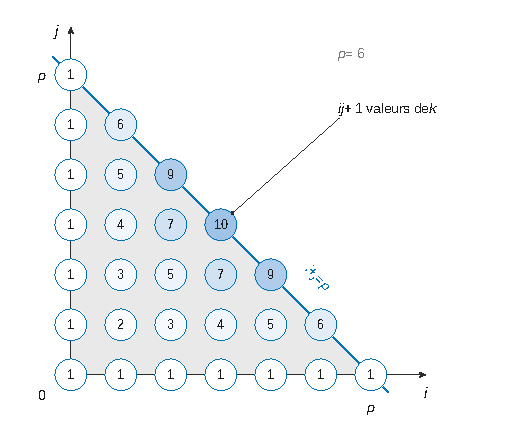
\includegraphics{figures/q40-denombrement-triangle.pdf}
\caption*{Figure 4 --- Q40 pour p = 6 : chaque point (i, j) du triangle i + j ≤ p
porte ij + 1 valeurs de k, et leur somme vaut 𝒩₆ = 98}
\end{figure}

Soit \(h(t)=t(1-t)^2\), continue sur \([0,1]\) et nulle en \(1\).

La somme \(\frac1p\sum_{i=0}^ph(i/p)\) est donc égale à \(\frac1p\sum_{i=0}^{p-1}h(i/p)\) : c'est une somme de Riemann, qui tend vers

\equationajustee{\begin{aligned}\int_0^1t(1-t)^2\,\mathrm{d}t&=\frac12-\frac23+\frac14\\&=\frac1{12}\neq0.\end{aligned}}

Donc

\equationajustee{\boxed{\frac{p^3}{2}\sum_{i=0}^p\frac ip\Bigl(1-\frac ip\Bigr)^2\underset{p\to+\infty}{\sim}\frac{p^4}{24}.}}

(Valeur exacte : \(\sum_{i=0}^pi(p-i)^2=\frac{p^2(p^2-1)}{12}\), donc la quantité vaut \(\frac{p^2(p^2-1)}{24}\).)

\hypertarget{q41}{%
\subsubsection{Q41}\label{q41}}

\emph{Majoration} : \(|{\mathcal{V}}_{\mathcal{A}}(p)|\leqslant32p^4\) pour \(p\geqslant1\) (Q38).

\emph{Minoration} : soit \((i,j,k)\in{\mathbb{N}}^3\) avec \(i+j\leqslant p\) et \(k\leqslant ij\). La condition de signe est satisfaite, donc \(f(i,j,k)\in{\mathcal{V}}_{\mathcal{A}}(p)\) (Q39).

Ces éléments sont distincts (\(f\) injective). Donc, par Q40,

\equationajustee{|{\mathcal{V}}_{\mathcal{A}}(p)|\geqslant{\mathcal{N}}_p\geqslant\frac{p^2(p^2-1)}{24}.}

Pour \(p\geqslant2\), on a \(p^2-1\geqslant\frac34p^2\), donc \(|{\mathcal{V}}_{\mathcal{A}}(p)|\geqslant\frac{p^4}{32}\).

Pour \(p=1\), \(|{\mathcal{V}}_{\mathcal{A}}(1)|=7\geqslant\frac1{32}\).

Ainsi \(\frac1{32}p^4\leqslant|{\mathcal{V}}_{\mathcal{A}}(p)|\leqslant32p^4\) pour tout \(p\geqslant1\), et par Q31 la propriété ne dépend pas de la partie génératrice :

\equationajustee{\boxed{\mathbb{H}\ \text{est un groupe \text{à} croissance polynomiale de \text{degré}}\ 4.}}

En particulier, bien qu'en bijection avec \({\mathbb{Z}}^3\), \(\mathbb{H}\) n'est pas isomorphe à \(({\mathbb{Z}}^3,+)\) (degré \(3\), Q32).

\end{document}
